% !TeX root =../../main.tex

\chapter{The FOT Fuzzing Framework} \label{ch:fot}


\section{Introduction and Motivation}


In spite of the popularity and effectiveness of applying greybox fuzzing techniques in detecting vulnerabilities(c.f. Sec~\ref{sec:intro-gbf}), there lacks a general fuzzing framework to reuse, integrate and evaluate various fuzzing extensions and~try new ideas.
For example, {\AFL}'s core fuzzing logic is implemented in one file with around 8K LOC, with more than 100 global variables. Therefore, the integration of a single new feature often involves modifications in multiple places.
In short, {\AFL} is highly coupled as it is designed to \textit{essentially require no configuration}~\cite{afl}.
In fact, most of the existing fuzzers are designed for easy deployment and use, without considering easy extension.
Hence, a fuzzing framework is preferred to allow for both easy \emph{configuration} and \emph{extension}.


Due to this, we propose our fuzzing framework, \emph{Fuzzing Orchestration Toolkit} ({\FOT}), which is designed to have the following three properties.

\begin{enumerate}[(1)]

\item  \textbf{Versatility.}
{\FOT} provides a fuzzing ecosystem, including a set of static and dynamic analysis toolchains to aid the fuzzing process.
\item \textbf{Configurability.}
{\FOT} provides multiple configurable options.	
Users can improve the fuzzing effectiveness with their experience by tweaking the parameters without development efforts.
\item \textbf{Extensibility.}
{\FOT} is of high coherence and low coupling. In fact, the implementation is composed of two parts: the library that contains general fuzzing utilities, and the miscellaneous tools on top of it. Therefore, apart from the default fuzzing tools provided by {\FOT}, developers may also write their own fuzzers with modest effort based on the library.
\end{enumerate}


\section{Architecture Design}\label{sec:details}

This section briefly describes the design of {\FOT} framework. Complementary results {\FOT} are available at ~\cite{fot-webpage}.


\begin{figure}[t]
	\centering
	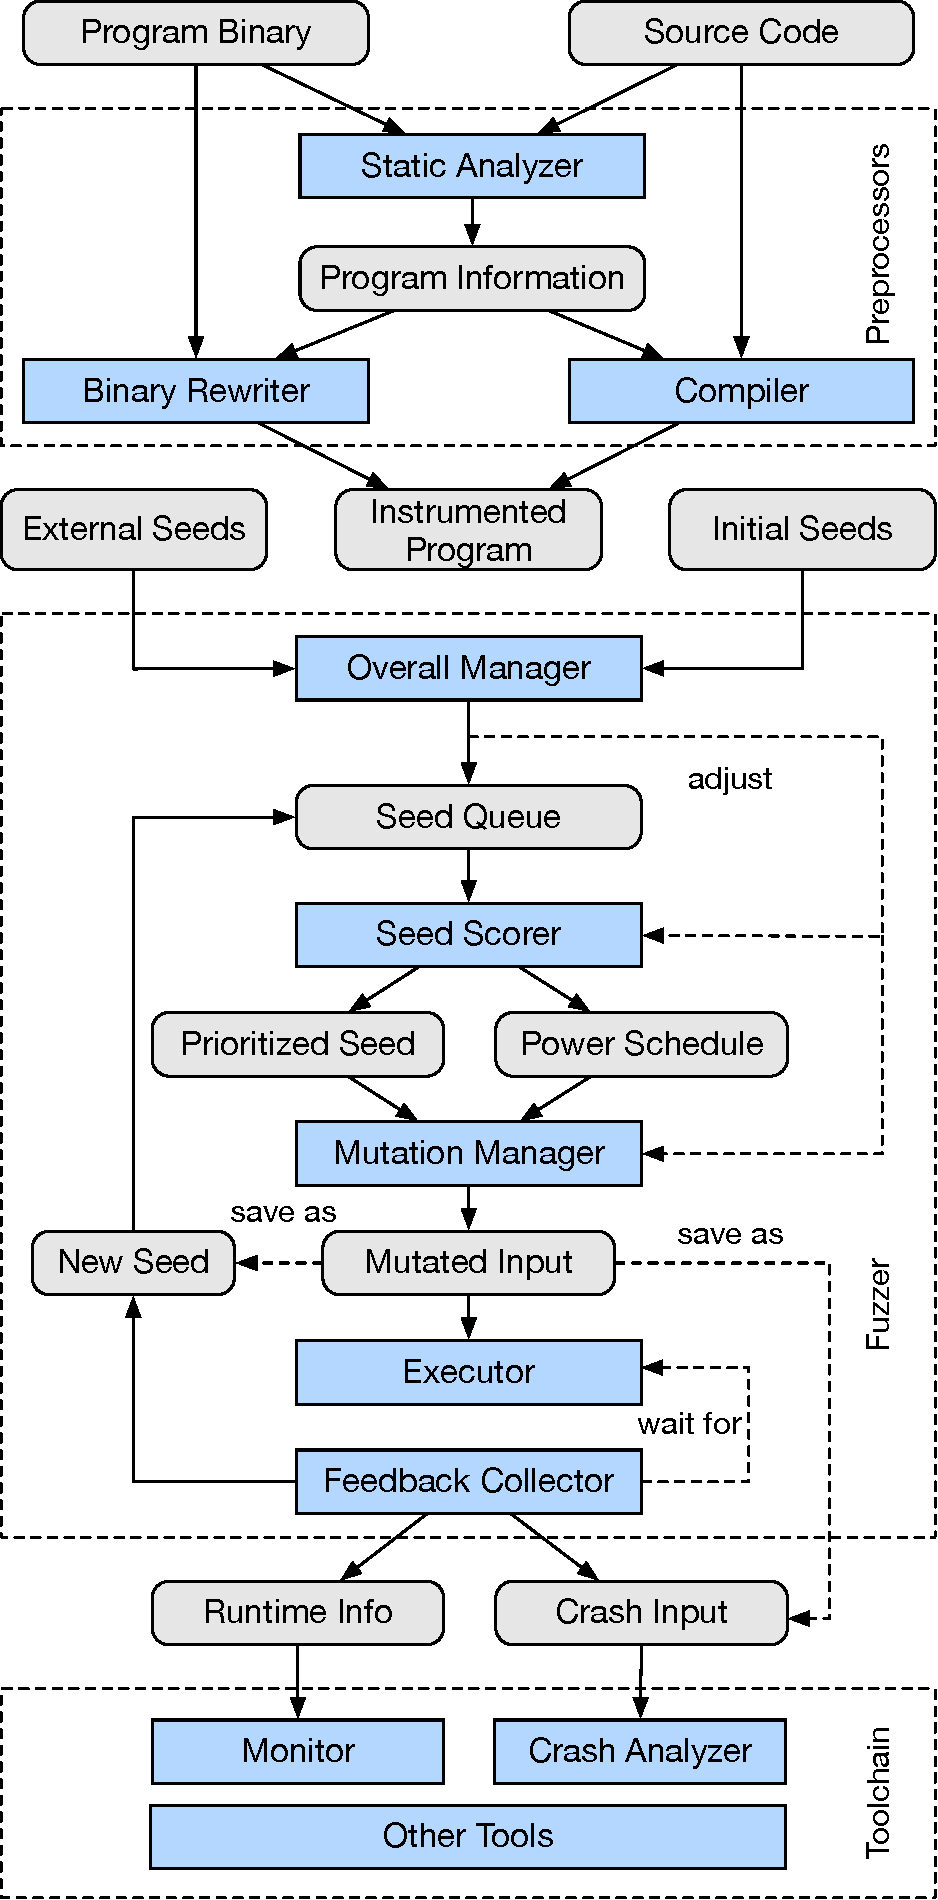
\includegraphics[width=0.64\textwidth]{res/fot/FOT_overview}
	\caption{Overview of the {\FOT} Fuzzing Framework}
	\label{fig:fot_workflow}
\end{figure}

Fig.~\ref{fig:fot_workflow} depicts the overview of {\FOT}.
It has three parts (labeled in pink): the \emph{preprocessor}, the \emph{fuzzer}, and the \emph{complementary toolchains}.
Components of the framework are represented with \emph{blue} rectangles while the inputs and outputs are in \emph{grey}. All these components inside \FOT are \textit{configurable} and \textit{extensible}.


\subsection{Preprocessor}
This contains various tools to collect static information and apply instrumentations.


\subsubsection{Static Analyzer}\label{sec:static_analysis}
It consists of tools to extract semantics from the PUT.
For example, we provide tools to generate the control flow graph, call graph or statically predicted vulnerabilities and convert them into proper representations which can be later instrumented into the PUT and utilized during dynamic fuzzing.
It is \textit{configurable} to generate different levels of static information. It is \textit{extensible} as developers are allowed to add new types of static analysis as long as the generated result follows the specified format.


\subsubsection{Instrumentor}
\emph{Binary rewriter} and \emph{source transformer} instrument static results generated by the static analyzer into the PUT for the fuzzer to collect feedback during runtime execution.
{\FOT} supports LLVM based instrumentation when program source is available, and Dyninst~\cite{dyninst} instrumentation when only the binary is given.
It is \textit{configurable} since the users can choose to instrument either on source code or binary.
It is \textit{extensible} since developers can use instrumentors such as Intel PIN~\cite{pin} as long as the instrumented code can embed the static information and provide sufficient feedback during fuzzing.

\subsection{Fuzzer}
This part explains the core fuzzing process. 
The fuzzer is essentially a loop that continuously selects seeds from a seed queue, applies mutations to the selected seeds, executes the PUT against mutated inputs, and collects statistics for the next iteration.

\subsubsection{Conductor}
As {\FOT} is designed to support multi-threaded parallel fuzzing, it contains the \emph{conductor} for fuzzing, scheduling the workload of different fuzzing instances.
Particularly, it monitor a special directory to actively import seed inputs from external tools such as symbolic executors (e.g., KLEE~\cite{klee}) or mutation generators (e.g., Radamsa~\cite{radamsa}).
It is \textit{configurable} since the users are allowed to choose different strategies for the overall management.
It is \textit{extensible} since it can interoperate with other external tools.


\subsubsection{Seed Scorer}
The seed scorer is in charge of selecting a seed from the queue for mutation (seed selection/prioritization) and determining how many new inputs should be generated based on the selected seed (power scheduling).
It is \textit{configurable} since the users can select from several built-in scoring strategies to evaluate seeds.
It is \textit{extensible} since the developers can implement their own strategies with the provided interfaces.


\subsubsection{Mutation Manager}
The mutation manager schedules different kinds of mutators.
It is \textit{configurable} as {\FOT} provides various mutators the their combinations for the users to select from.
It is \textit{extensible} as the developers can implement their own mutators with the provided interfaces.

\subsubsection{Executor}
The executor drives the execution of the PUT.
It is \textit{configurable} since the default executor in {\FOT} allows users to choose whether or not to use forkserver~\cite{afl} during fuzzing.
It is \textit{extensible} since the developers can extend the executor for various scenarios.
For example, they may add a secondary executor to execute another PUT for differential testing.

\subsubsection{Feedback Collector}
The feedback collector collects the feedback emitted by the PUT.
The exact feedback often corresponds to the instrumented information.
It is \textit{configurable} as the users are allowed to select from the default feedback options provided by {\FOT}.
For now, the feedback can be at basic-block level (like {\AFL}) or function level.
It is \textit{extensible} as the users can specify their customized types of feedback for collection.

\subsection{Complementary Toolchain}
{\FOT} contains various tools helping to make the framework \textit{versatile}.
For instance, we implemented a web-based frontend user interface to monitor the overall results.
It provides fruitful information to make the fuzzing process more transparent.
We also provided a crash analyzer to analyze the detected crashes and automatically generate reports.
This greatly reduces the manual efforts of crash triaging.
Many other extensions are also being added to complement the fuzzer.


\begin{figure}[t]
	\centering
	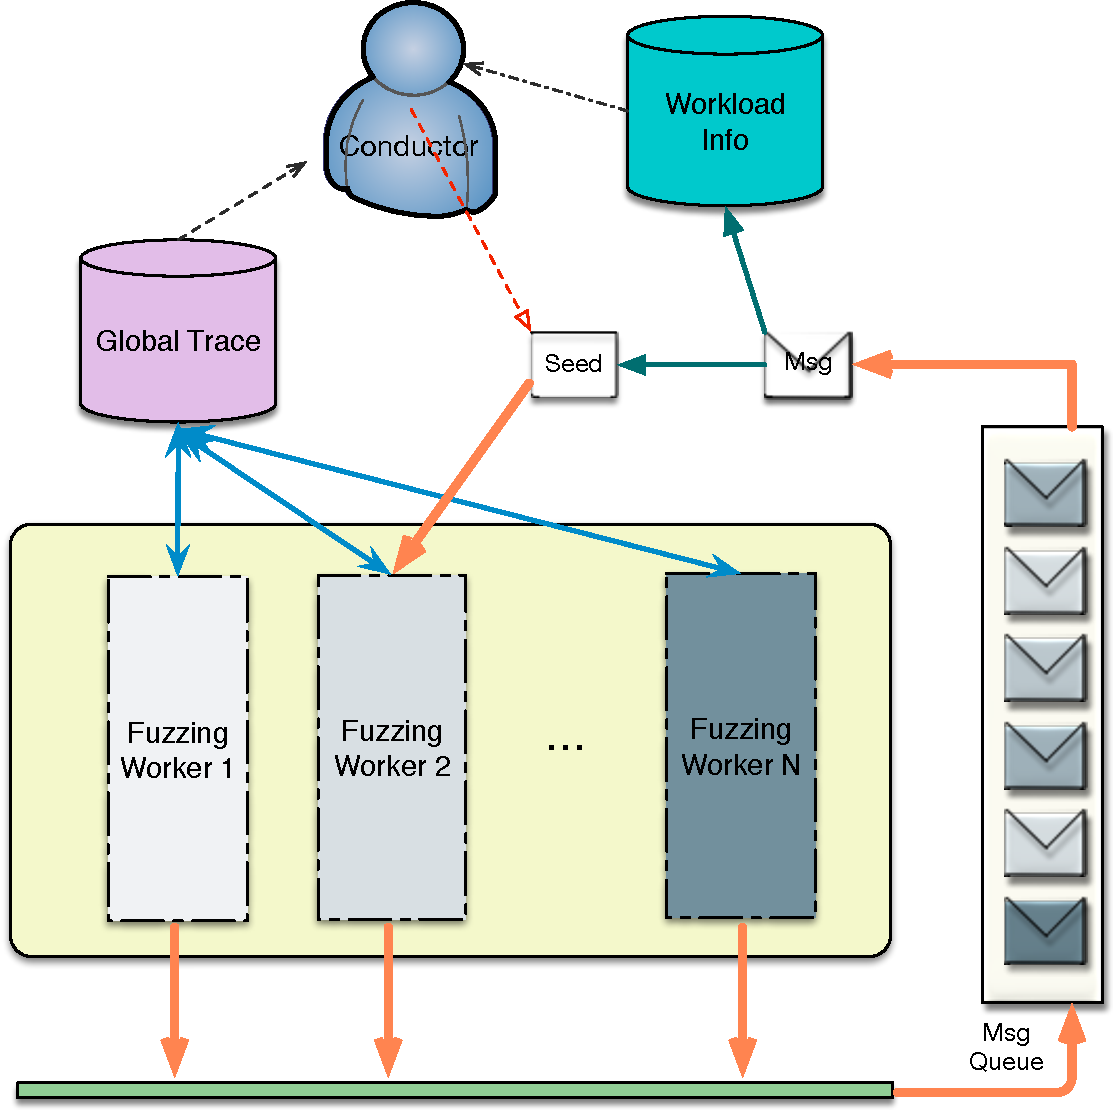
\includegraphics[width=0.6\columnwidth]{res/fot/mt_workflow}
	\caption{Coordination among Different Fuzzing Instances}
	\label{fig:mt_workflow}
\end{figure}


\subsection{Trace Update and Synchronization}\label{sec:trace_sync}
One of {\FOT}'s key features is the builtin coordination among different fuzzing instances (Fig.~\ref{fig:mt_workflow}). One important issue is the trace synchronization between fuzzing instances. For instrumentation, we made a slight change to the conventional instrumentation runtime to make the target binaries able to distinguish different shared memory arenas and the file descriptors used for ``forkserver'' allocated/specified by different fuzzing workers. Each fuzzing worker allocates the shared memory and the instrumented binary writes to specific multiple 8-byte areas when the corresponding ``execution edges'' have been reached. By auditing the byte fingerprints, the fuzzer knows about the edges and their approximate hit counts within this run. This information sits between between ``branch coverage'' and ``path coverage''. By comparing the shared memory fingerprint with the local trace information (checking whether the active shared memory byte has been marked ``traced'' locally), the fuzzer gets the knowledge whether current running seed increases the coverage. Updating of the local trace is majorly a ``bitwise and'' where each byte of the local trace is initialized with all ones (i.e., 255).

The local trace is synchronized with the global trace state. There stands a tradeoff: if we use directly the global trace state, the synchronization will be too frequent and eventually decreases performance with the increase of more fuzzing workers; if the fuzzers are only aware of the local trace, it is no better than {\AFL}'s na\"ive approach that runs all instances separately. We thus choose to only apply the synchronization during the mutation of each test case in the queue, when customizable conditions are triggered (usually the conditions are about the executions and time since last synchronization).

The actual synchronization of the trace information still applies ``bitwise and'' on normal running traces from local trace information to global state, and an instant copy in the other direction. This is far more efficient than {\AFL}'s synchronization by 1) importing seeds from other directories and 2) running all the test cases indistinguishably. Note that {\FOT}'s synchronization does not lose precisions compared to {\AFL}'s, where both ``bitwise and'' operations erase the exact hit count information.


  \subsection{Mutation Strategy Adaption}\label{sec:mutation_ops}
 The selection of mutation operators during fuzzing on one test input is determined by two factors:
 \begin{enumerate}
 	\item The whitelist mutation operators used for the targeted binaries. Some mutation operators are only effective on certain programs, but is almost a waste of time for the other programs (for example, bitflip operations are quite expensive and rarely useful for text-based parser programs running against large files). This can be specified by the experienced {\FOT} users.
 	\item The one-time mutation operators for \emph{this fuzz}. This is automatically determined by the fuzzer according to statistics generated from the previous mutations and runs. It is calculated in an adaptive way and may finally help to determine the ``convergence'' of the test cases.
 \end{enumerate}

On the other hand, being super general, {\AFL} has limited configurations for what mutation operators can be used and frequently runs blindly on the mutations that do not fit well~\cite{junjie:2017sp:skyfire,mopt-fuzz}.


\subsection{Refinement on Variable Behaviors}\label{sec:entry_var_behavior}

Some programs have variable behaviors for the same input test, due to randomness, multi-threading, etc. {\AFL} handles this issue by running all the newly found interesting test cases multiple times (known as \emph{calibration}); whenever it finds that the shared memory information (the active bytes and their hit count) differs from the first run, it will give more chances to the running test entry, and then keeps track of the variable behavior rate. The problem is that it does not utilize the information further since variable behaviors may cause certain runs to exit normally at some time, however crash at other time, which is more serious. We separately track those test case and give even more chances for these seeds. Alternatively, we provide an intrinsic strategy to prioritize these cases and let those test cases to be more likely to run next time. On the other hand, {\AFL}'s tracing information for the variable behavior cases are imprecise since it only traces the last calibration shared memory; we refine this by (selective) ``bitwise or'' operations to the shared memory for subsequent procedures on the current seed.


 \subsection{Trimming on Duplicated Cases}
Due to the existence of the potential lag of the trace synchronization, there still exists test input that runs with the same running trace. In other cases, the test cases might not be in its ``simplest'' form: by removing some bytes, the input test case can still results in the same running trace. {\FOT}'s approach in handling this is to trim the calibrated test cases immediately before being parceled as the message and sent to the message queue buffer managed by the conductor. And the conductor maintains a checksum set of all the generated seed files. Therefore when the newly generated seed has the same checksum as one of the existing ones, this test case will be discarded.

Additionally, we provide an external minimizer program to prune the all the serialized test cases (which can be normal runs, timeout runs, or crashes); it is more aggressive than the embedded procedure in the fuzzer and aims to provide a minimized version of all the interesting test cases.
 

\subsection{Implementation}\label{sec:fot-impl}

The {\FOT} project started from June, 2017 and has been actively developed by two researchers. It is implemented with 16000 lines of Rust for core fuzzing modules, together with 4500 lines of C/C++ for the preprocessor, 4200 lines of Java for structure-aware mutation, and 2400 lines of Python for complementary toolchain.
  

\section{Comparisons to Other Fuzzing Frameworks and Extensions}


In this section, we first compare FOT with other fuzzing frameworks, and then discuss its relationship to current fuzzing extensions.



Table~\ref{tbl:cmp_fuzz} compares {\FOT} with existing fuzzing frameworks with respect to 10 major features. As we can see, the existing fuzzing frameworks AFL, libFuzzer and honggfuzz lack \FOT's features in various aspects. {\FOT} stands out in that it provides multiple configurations for advanced users; it is also highly modularized, suitable to be extended with other fuzzing techniques. Moreover, {\FOT} partially supports structure-aware mutations and interoperability with other external tools such as symbolic executors (by monitoring and scheduling newly incoming seed input directory).

Most current fuzzing extensions can be easily integrated into {\FOT} owing to its design. In reality, they can be applied with some extensions to the different components in Figure~\ref{fig:fot_workflow} and can be used together with the configuration interface. 

\begin{enumerate}[1)]
	\item AFLFast~\cite{Bohme:2016:CGF} can be implemented by applying a Markov Chain model based seed \emph{power scheduling} in the fuzzer. 
	\item AFLGo~\cite{Bohme:2017:DGF} can be implemented by a combination of \emph{static analyzer}, \emph{instrumentation} and \emph{power scheduling}.
	\item CollAFL~\cite{CollAFL} can be implemented by using a collision-resistant algorithm to increase the uniqueness of the path trace labeling during \emph{instrumentation}.
	\item Skyfire~\cite{junjie:2017sp:skyfire}, Radamsa~\cite{radamsa}, Csmith~\cite{csmith} can be used in the preprocessor to generate seeds for the \emph{external seeds} and a structure-aware mutator assigned by \emph{mutation manager}.
	\item Symbolic executors such as KLEE~\cite{klee} can be integrated in the Driller's~\cite{driller} style with the help of \emph{conductor}.
\end{enumerate}

\begin{table}[t]
\centering
	\small
	\caption{Comparisons between fuzzing frameworks (\Circle: not supported, \LEFTcircle: partially supported, \CIRCLE: fully supported)}
	\label{tbl:cmp_fuzz}
	\begin{tabular}{|l|c|c|c|c|}
		\hline
		\diagbox{\textbf{Features}}{\textbf{Framework}} & \textbf{AFL} & \textbf{libFuzzer} & \textbf{honggfuzz} & \textbf{FOT} \\ \hline\hline
		Binary-Fuzzing Support & \CIRCLE & \Circle & \CIRCLE & \CIRCLE \\ \hline
		Multi-threading Mode & \Circle & \CIRCLE  & \CIRCLE  & \CIRCLE  \\ \hline
		In-memory Fuzzing &\CIRCLE  & \CIRCLE &\CIRCLE  & \CIRCLE \\ \hline
		Advanced Configuration & \Circle  & \LEFTcircle  & \Circle  & \CIRCLE  \\ \hline
		Modularized Functionality & \Circle & \LEFTcircle & \Circle & \CIRCLE \\ \hline
		Structure-aware Mutation & \Circle  &\Circle & \Circle  & \LEFTcircle \\ \hline
		Interoperability & \Circle & \Circle & \Circle & \LEFTcircle \\
		\hline
		Toolchain Support &  \CIRCLE & \Circle  & \Circle  & \CIRCLE \\ \hline
		Precise Crash Analysis & \Circle  & \Circle  & \CIRCLE  & \CIRCLE  \\ \hline
		Runtime Visualization & \LEFTcircle & \Circle & \Circle & \CIRCLE \\ \hline
	\end{tabular}
\end{table}


\subsection{New Vulnerabilities}

At the time of writing, {\FOT} has been used to fuzz more than 100 widely used open source projects and it has detected more than 200 vulnerabilities, among these 51 CVE IDs have been assigned. The detailed information is available at Appendix~\ref{app:bugs}. Notably, \FOT has detected multiple vulnerabilities with \emph{high} or \emph{critical} severity. For example, CVE-2019-9169~\cite{CVE-2019-9169} stresses a vulnerability in the GNU C Library (a.k.a glibc or libc6 on Linux distributions) through 2.29, where the function \func{proceed\_next\_node} inside POSIX regular expression (regex) component has a heap-based buffer over-read via an attempted case-insensitive regex match. Thanks to the interoperability with the regex generators, FOT is able to generate more meaningful seeds that cover more corner cases of the regex components. According to CVSS v3.0 Severity and Metrics~\cite{cvss3}, it is scored 9.8 out of 10.0 (critical severity); according to CVSS v2.0~\cite{cvss2}, it has a score of 7.5 (high severity). As a comparison, the notorious HeartBleed (CVE-2014-0160) is scored 5.0 medium severity according to CVSS v2.0 (there is no CVSS v3.0 for it). Many of other vulnerabilities discovered by \FOT also have high severity, e.g, CVE-2018-15822, CVE-2018-14394, CVE-2018-14395 in FFmpeg, CVE-2018-19837, CVE-2018-19838, CVE-2018-19839, CVE-2018-20821, CVE-2018-20822 in libsass, CVE-2018-14560, CVE-2018-14561, CVE-2019-11470, CVE-2019-11472 in ImageMagick, and CVE-2019-11473, CVE-2019-11474 in GraphicsMagick. We envision that with more integrated fuzzing techniques, \FOT will have the capabilities to detect more vulnerabilities that are hard to be discovered by existing fuzzers.
